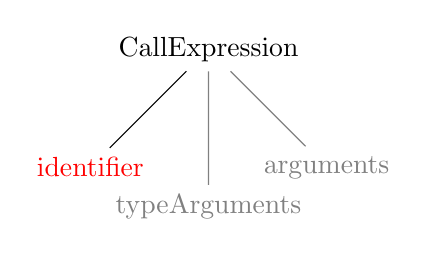
\begin{tikzpicture}
	\node {CallExpression}
		child {node [red] {identifier}}
		child [gray] {node [gray, yshift = -0.5cm] {typeArguments}}
		child [gray] {node [gray] {arguments}};
\end{tikzpicture}
\caption[LoF entry]{
	Node pattern for a TypeScript functional call, such as in:

	\code{\lowlight{result = }\uline{\highlight{fun}<\lowlight{T1}, \lowlight{T2}>(\lowlight{arg1}, \lowlight{arg2})}\lowlight{;}}
}
